\normaltrue
\correctiontrue

%\UPSTIidClasse{11} % 11 sup, 12 spé
%\newcommand{\UPSTIidClasse}{12}


\exer{Mouvement T -- $\star$ \label{CIN:01:B2:12:01}}
\setcounter{question}{0}\marginnote{\xpComp{CIN}{01}}%\UPSTIcompetence{B2-12}
\index{Compétence B2-12}\index{Compétence CIN-01}
\index{Mécanisme à 1 translation}
\ifcorrection
\else
\marginnote{\textbf{Pas de corrigé pour cet exercice.}}
\fi

\ifprof
\else
Soit le mécanisme suivant. On note $\vect{AB}=\lambda(t)\vect{i_0}$.
\begin{marginfigure}
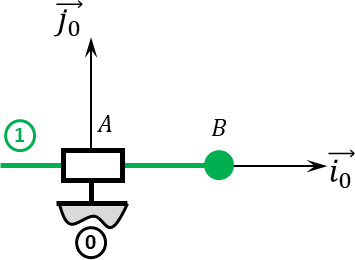
\includegraphics[width=\linewidth]{01_T_01}
\end{marginfigure}
\fi

\ifprof
\begin{multicols}{3}
\else
\fi
\question{Tracer le graphe des liaisons.}
\ifprof\begin{marginfigure}
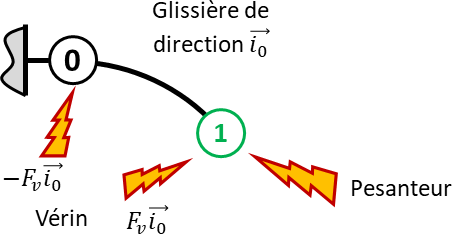
\includegraphics[width=\linewidth]{01_T_01_c}
\end{marginfigure}
\else
\fi


\question{Retracer le schéma cinématique pour $\lambda=\SI{10}{mm}$.}
\ifprof
\begin{marginfigure}
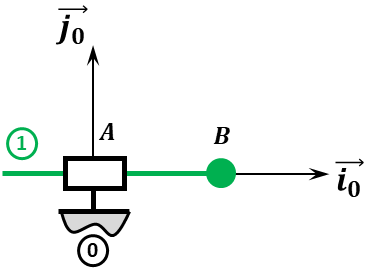
\includegraphics[width=\linewidth]{01_T_02_c}
\end{marginfigure}
\else
\fi

\question{Retracer le schéma cinématique pour $\lambda=-\SI{20}{mm}$.}
\ifprof
\begin{marginfigure}
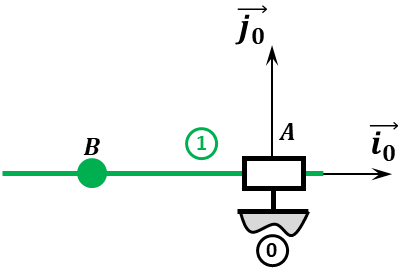
\includegraphics[width=\linewidth]{01_T_03_c}
\end{marginfigure}
\else
\fi


\ifprof
\end{multicols}
\else
\fi

\ifprof
\else

\marginnote{Corrigé  voir \ref{CIN:01:B2:12:01}.}

\fi


